% !TEX program = xelatex
\documentclass[11pt]{article}
\usepackage[margin=1in]{geometry}
\usepackage{nopageno} % no page numbers
\usepackage{setspace}

\usepackage{graphicx}
\graphicspath{ {./graphics/} }
\usepackage[dvipsnames]{xcolor}
\definecolor{CrispBlue}{HTML}{0176AE}

\usepackage{fontspec}
\usepackage{tcolorbox}
\usepackage{etoolbox}
\BeforeBeginEnvironment{verbatim*}{\begin{tcolorbox}[colback=CrispBlue!5!white,colframe=CrispBlue!75!black]}%
\AfterEndEnvironment{verbatim*}{\end{tcolorbox}}%

\usepackage{hyperref}
\hypersetup{
    colorlinks,
    citecolor=black,
    filecolor=black,
    linkcolor=black,
    urlcolor=black
}

\usepackage{subcaption}
\setlength{\parindent}{0pt}
\setlength{\parskip}{1em}

\usepackage{tocloft}
\renewcommand{\cftpartleader}{\cftdotfill{\cftdotsep}}
\renewcommand{\cftsecleader}{\cftdotfill{\cftdotsep}}

\usepackage{fancyhdr}
\pagestyle{fancy}
\fancyhf{}
\lhead{ECE 517: Machine Learning}
\rhead{Assignment 6.1}
\rfoot{Page \thepage}

\usepackage{amsmath,amsfonts,amssymb}
\usepackage{bm}
\usepackage{mathtools}

\renewcommand{\listfigurename}{List of Figures}

\begin{document}
\setmainfont{SF Pro Text}
\setsansfont{SF Pro Text}
\setmonofont{SF Mono}
\renewcommand{\familydefault}{\sfdefault}

\thispagestyle{empty}
\begin{titlepage}
\vspace*{\fill}
\begin{center}
\textsc{\Huge{ECE 517: Machine Learning}}\\[3em]
\textsc{\LARGE Assignment 6.1: Primal Formulation of a Nonlinear\\[0.5em]Classifier With MMSE}\\[6em]
\textsc{\Large David Kirby -- 101652098 -- davidkirby@unm.edu}\\[3em]
\textsc{\Large Fall 2021}
\end{center}
\vfill
\begin{figure}[h]
\begin{subfigure}{0.5\textwidth}

\includegraphics[width=0.25\linewidth]{learning.png}
\end{subfigure}
\begin{subfigure}{0.6\textwidth}\hspace{1em}

\includegraphics[width=0.8\linewidth]{new-soe-logo.png}
\end{subfigure}
\end{figure}
\end{titlepage}
\setcounter{figure}{0}

\hypersetup{
    linkcolor=CrispBlue,
    urlcolor=CrispBlue,
    breaklinks=true
}

\textbf{PRIMAL FORMULATION OF A NONLINEAR CLASSIFIER WITH MMSE}

Use the attached function to reconstruct the example of lesson 6.1. In particular, you must:

\begin{enumerate}
    \item Construct a train dataset and represent them. Your representation may be rotated 90º with respect to the one of the slides.
    \item Construct a function to directly map the data into a 10 dimension Hilbert space using the Volterra expansion.
    \item Compute the weights of the MMSE solution, and represent the boundary as indicated in the slides.
\end{enumerate}

Provide a document that summarizes the theory and a graph of the result. Comment your results.

[Code omitted for brevity.]
% \begin{verbatim}
%     %%% MATLAB CODE %%%

%     [X,y]=data(100,0.2)

%     i1=find(y==1);
%     i2=find(y==-1);
%     figure(1)
%     plot(X(1,i1),X(2,i1),'s')
%     hold on
%     plot(X(1,i2),X(2,i2),'r*')
%     xlabel('x[n-1]')
%     ylabel('x[n]')

%     function [X,y]=data(N,a)
%     N=N+1;
%     y=sign(randn(1,N));
%     x=filter([1 a],1,y)+0.2*randn(size(y));
%     X=buffer(x,2,1,'nodelay'); %Convolution
%     y=y(2:end)
%     end
% \end{verbatim}

\begin{tcolorbox}[colback=CrispBlue!5!white,colframe=CrispBlue!75!black,title=Primal formulation of a non-linear classifier with MMSE.]\setstretch{1.25}

This problem takes a linear channel and solves it using a non-linear approach consisting of transforming our data into a higher dimensional Hilbert space (a higher dimensional vector space). One way to do this is with the Volterra expansion which computes products of the different features of our vector. We have a vector of two components, which in our case is \(x[n]\) and \(x[n-1]\), and we compute combinations of products up to a third order. With this, we have ten dimensions, including one where we have a cost. Then, we put all these components into a new vector of ten components and we apply the Minimum Mean Square Error approach. So, \(\mathbf{w}\) has the same solution as in our previous lectures, but instead of having \(\mathbf{x}_n\), we have \(\Phi\), where \(\Phi\) is a matrix containing all the values of the transformed vector.
\begin{equation}
    \mathbf{w} = (\Phi \Phi ^\top)^{-1} \Phi y
\end{equation}

Adjusting the parameters following this algorithm, we can represent points defined by the hyperplane \( \mathbf{w}^\top \phi (x_n) = 0\) and these points are the boundary (as shown in Figure~\ref{fig:figure02}) that non-linearly classify almost all points.\\

The problem is that we have ten dimensions for an input of two dimensions. For example, if we use an expansion with order five, then we would need 56 elements, and so on. This is what we call the curse of dimensionality. If we want a solution that works better than this example, which is not very efficient, we need to add more expressive capacity to our machine by using a space with more dimensions. In other words, we have to increase the Vapnik--Chervonenkis dimension on that space.

\end{tcolorbox}

\begin{figure}[h!]
    \centering
    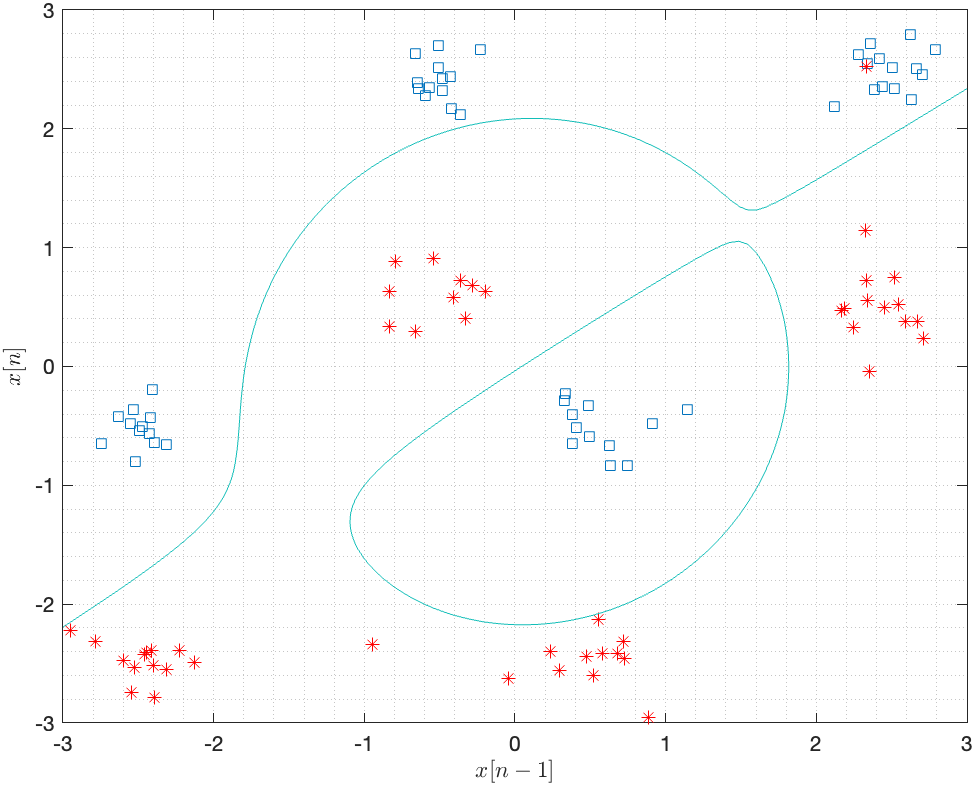
\includegraphics[width=\textwidth]{figure02.png}
    \vspace{1em}\caption{Computed weights of the MMSE solution and representation of the boundary.}
    \label{fig:figure02}
\end{figure}

\end{document}